\documentclass{beamer}
\usepackage{multicol}
\usepackage{xy}
\everymath{\displaystyle}
\mode<presentation>
{\usetheme{Warsaw}\setbeamercovered{dynamic}}
\usecolortheme{crane}
\usepackage{beamerfoils}
\pgfdeclareimage[height=1in]{university-logo}{ISULogo}
\logo{\pgfuseimage{university-logo}}
\setbeamertemplate{navigation symbols}{}
\title[\S8]{Section 8\\The Counting Principle and permutations}
\author{Dr Marcus Bishop}
\subject{Math 104}
\beamerdefaultoverlayspecification{<+->}
\theoremstyle{definition}
\newtheorem{remark}{Remark}
\newtheorem{impact}{Impact}
\newtheorem{notation}{Notation}
\newtheorem{argument}{Argument}
\usepackage{arev}
\begin{document}
\begin{frame}\titlepage\end{frame}
\LogoOff

\begin{frame}
{What I do outside of class that helps me learn}
(Selected comments from course evaluations
paraphrased slightly to improve humor and style)
\begin{itemize}
\item Homework, study guide problems, past exams, slides,
YouTube videos
\item Math help room, Josh's office hours, instructor's office hours,
private tutors
\item Study with friends, organize or attend study groups
\item I tutor my friends;
this helps me to understand the material better because
it forces me to know it well enough to teach others.
\item I always travel with friends at night, because I'm afraid the
instructor will jump out from behind a tree and make me do Venn diagrams
\end{itemize}
\end{frame}

\begin{frame}{What I like about Math 104}
\begin{itemize}
\item Professor is funny, entertaining, energetic, upbeat
\item Frequency, easiness, amount of homework
\item I don't enjoy anything about Math 104
\item I enjoy learning about casino games
\item Math 104 lectures resemble
getting a root canal, except that it only lasts 50 minutes, hallelujah!
\item Material interesting, useful, applicable to real world
\item Class might feel like being lost at sea,
but at least my friends are all here with me!
\end{itemize}
\end{frame}

\begin{frame}{What I would change about Math 104}
\begin{itemize}
\item The instructor; I'd say my cat could teach the
course better, and he's actually looking for a job!
\item Instructor better prepared, organized, competent
\item More examples, explained slower, in greater depth
\item Lectures too slow
\item Lectures too fast
\item Homework submission, retrieval, exam distribution
\item Use Blackboard calendar
\item Exams and quizzes harder than homework
\item Instructor reads slides aloud
\end{itemize}
\end{frame}

\begin{frame}{Permutations}
\begin{itemize}
\item Ways of arranging set of distinct objects called
\alert{permutations}, \alert{arrangements}, or \alert{anagrams}
%\item Objects meant to be arranged linearly
\item Order matters in listing permutations
\begin{example} Six permutations of $\left\{1,2,3\right\}$:
\[123\quad 132\quad 213\quad 231\quad 312\quad 321\]
\end{example}
\item Permutations can be generated using tree diagram:
\only<+->{
\[\begin{xy}<1cm,0cm>:
(0,0)="0";
(-3,-1)="-31";
(0,-1)="01";
(3,-1)="31";
"0";"-31"*+!D{1}**\dir{-};
"0";"01"*+!D{2}**\dir{-};
"0";"31"*+!D{3}**\dir{-};
"-31";(-4,-2)*+!D{2}**\dir{-};
(-4,-3)*+!D{3}**\dir{-};
"-31";(-2,-2)*+!D{3}**\dir{-};
(-2,-3)*+!D{2}**\dir{-};
"01";(-1,-2)*+!D{1}**\dir{-};
(-1,-3)*+!D{3}**\dir{-};
"01";(1,-2)*+!D{3}**\dir{-};
(1,-3)*+!D{1}**\dir{-};
"31";(2,-2)*+!D{1}**\dir{-};
(2,-3)*+!D{2}**\dir{-};
"31";(4,-2)*+!D{2}**\dir{-};
(4,-3)*+!D{1}**\dir{-};
\end{xy}\]}
\end{itemize}
\end{frame}

\begin{frame}
\begin{itemize}
\item But drawing tree inefficient when only
\alert{number} of permutations needed
\item Observe that tree has $3$~branches,
each with $2$~branches, each with $1$~leaf
\item So $3\cdot 2\cdot 1=6$ leaves
\[\begin{xy}<1cm,0cm>:
(0,0)="0";
(-3,-1)="-31";
(0,-1)="01";
(3,-1)="31";
"0";"-31"*+!D{1}**\dir{-};
"0";"01"*+!D{2}**\dir{-};
"0";"31"*+!D{3}**\dir{-};
"-31";(-4,-2)*+!D{2}**\dir{-};
(-4,-3)*+!D{3}**\dir{-};
"-31";(-2,-2)*+!D{3}**\dir{-};
(-2,-3)*+!D{2}**\dir{-};
"01";(-1,-2)*+!D{1}**\dir{-};
(-1,-3)*+!D{3}**\dir{-};
"01";(1,-2)*+!D{3}**\dir{-};
(1,-3)*+!D{1}**\dir{-};
"31";(2,-2)*+!D{1}**\dir{-};
(2,-3)*+!D{2}**\dir{-};
"31";(4,-2)*+!D{2}**\dir{-};
(4,-3)*+!D{1}**\dir{-};
\end{xy}\]
\item Could use same mechanism to count permutations
of $\left\{1,2,3,4\right\}$ without drawing tree
\item Tree would have $4$~branches, each with $3$~branches,
each with $2$~branches, each with $1$~leaf
\item So tree would have $4\cdot 3\cdot 2\cdot 1=24$ leaves
\item So $24$ the number of permutations of four objects
\end{itemize}
\end{frame}

\begin{frame}{Factorial}
\begin{itemize}
\item Similarly $120=5\cdot 4\cdot 3\cdot 2\cdot 1$
the number of permutations of $5$ objects
\item In general $n\cdot\left(n-1\right)\cdot\left(n-2\right)
\cdots 3\cdot 2\cdot 1$ the number of permutations of $n$~objects
\item This number denoted by $n!$
\item $n!$ pronounced \alert{$n$ factorial}
\item So $n!$ the number of permutations of $n$~objects
\end{itemize}
\end{frame}

\begin{frame}{Example from literature}
Murphy took the biscuits carefully out of the packet and laid them face
upward on the grass, in order as he felt of edibility. They were
the same as always, a Ginger, an Osborne, a Digestive, a Petit
Beurre and one anonymous. He always ate the first-named last, because
he liked it the best, and the anonymous first, because he thought
it very likely the least palatable. The order in which he ate the
remaining three was indifferent to him and varied irregularly from
day to day. On his knees now before the five it struck him for the
first time that this reduced to a paltry six the number of ways in
which he could make his meal.
\end{frame}
\begin{frame}
\dots Even if he conquered his
prejudice against the anonymous, still there would be only twenty-four
ways in which the biscuits could be eaten. But were he to take the
final step and overcome his infatuation with the ginger, then the
assortment would spring to life before him, dancing the radiant
measure of its total permutability, edible in a hundred and twenty
ways!\\
\hfill
from {\em Murphy} by Samuel Beckett
\end{frame}

\begin{frame}{Partial permutations}
\begin{itemize}
\item How many ways to arrange $6$ books on shelf?
\item $6!=6\cdot 5\cdot 4\cdot 3\cdot 2\cdot 1=720$
\item But what if shelf only has room for $3$ books?
\item Drawing tree cumbersome
\item If drawn, tree would have $6$~branches,
each with $5$~branches, each with $4$~leaves
\item Thus books can be arranged in $6\cdot 5\cdot 4=120$ ways
\item Slick way to write answer:
\[6\cdot 5\cdot 4
\only<+->{=\frac{6\cdot 5\cdot 4\cdot 3\cdot 2\cdot 1}
{3\cdot 2\cdot 1}}\only<+->{=\frac{6!}{3!}}
\only<+->{=\frac{6!}{\left(6-3\right)!}}\]
\item In general
$\frac{n!}{\left(n-r\right)!}$ the number of \alert{permutations
of $n$~objects taken $r$~at a time}
\item $\frac{n!}{\left(n-r\right)!}$ denoted
by $_nP_r$
\end{itemize}
\end{frame}

\begin{frame}
\begin{example}
\begin{itemize}
\item Number of ways to arrange $6$~books
on shelf, taken from set of $10$~books:
\item $_{10}P_6
\only<+->{=\frac{10!}{\left(10-6\right)!}}
\only<+->{=\frac{10!}{4!}}
\only<+->{=10\cdot 9\cdot 8\cdot 7\cdot 6\cdot 5}
\only<+->{=151,200}$
\item Observe that $\frac{10!}{4!}$ faster to type
on calculator than 
$10\cdot 9\cdot 8\cdot 7\cdot 6\cdot 5$, if calculator
has $!$ button
\end{itemize}
\end{example}
\begin{example}
\begin{itemize}
\item Number of ways to select president, vice president,
and treasurer from among Alex, Brooke, Colby, and Denise:
\item $_4P_3
\only<+->{=\frac{4!}{\left(4-3\right)!}}
\only<+->{=4\cdot 3\cdot 2}
\only<+->{=24}$
\end{itemize}
\end{example}
\end{frame}

\begin{frame}{Counting principle}
\begin{itemize}
\item In general, to count ways task can be performed
\begin{itemize}
\item Organize task into stages
\item At each stage, a single decision should be made
\item Calculate number of ways decision can
be made at each stage
\item Multiply numbers
\end{itemize}
\item Division of task into ``stages'' sometimes unnatural
\begin{example}
\begin{itemize}
\item Consider example with Alex, Brooke, Colby, and Denise
\item First stage: select president
\item Can be done in $4$ ways
\item Second stage: select vice president
\item Can be done in $3$ ways, since one person already
chosen for president at this stage
\item Et cetera
\end{itemize}
\end{example}
\end{itemize}
\end{frame}

\begin{frame}{ATM PINs}
\begin{itemize}
\item An Automated Teller Machine (ATM)
allows bank customers to withdraw money from accounts
\item Customer must enter secret $4$-digit
Personal Identification Number (PIN)
\item Inventor John Shephard-Barron of ATM envisioned $6$-digit PINs
\item However, his wife preferred $4$-digit PINs
\begin{example}
\begin{itemize}
\item How many $4$-digit PINs possible?
\item First stage: choose first digit, \only<+->{can be done in $10$ ways}
\item Second stage: choose second digit, \only<+->{can be done in $10$ ways}
\item Similarly for third and fourth digits
\item So $10\cdot 10\cdot 10\cdot 10\only<+->{=10^4}$
\only<+->{$=10,000$ PINs possible}
\end{itemize}
\end{example}
\end{itemize}
\end{frame}

\begin{frame}{Iowa license plates}
\begin{multicols}{2}
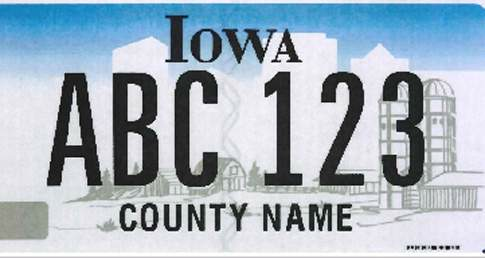
\includegraphics[scale=.3]{LicencePlate}
\begin{itemize}
\item Iowa license plates have three letters
and three digits
\item How many possible?
\item $26$ choices for first letter
\columnbreak
\item $26$ choices for second and third letters
\item $10$ choices for each of three digits
\item Thus $26\cdot 26\cdot 26\cdot 10\cdot 10\cdot 10$
\only<+->{$17,576,000$ plates possible}
\item Exceeds population of Iowa, $\approx 3,0000,000$
\end{itemize}
\end{multicols}
\end{frame}

\begin{frame}{Iowa area codes}
\begin{multicols}{2}
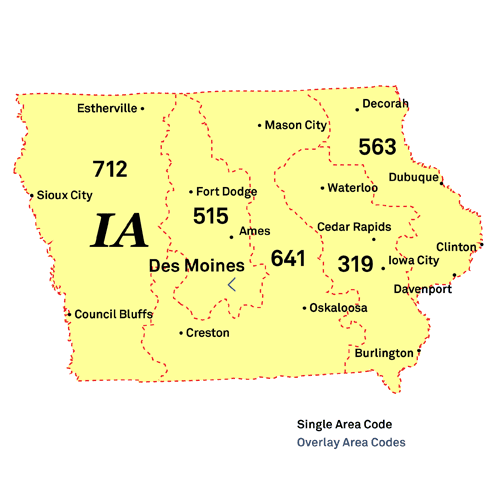
\includegraphics[scale=.35]{Iowa}
\begin{itemize}
\item Before 2000 Iowa had area codes $712$, $515$, and $319$
\item In 2000 Iowa introduced $641$ and $563$ due to increased usage
\item How many phone numbers within an area code?
\end{itemize}
\end{multicols}
\end{frame}

\begin{frame}{Phone numbers}
\begin{itemize}
\item Under North American Numbering Plan (NANP)
phone numbers consist of 
\begin{itemize}
\item three digit \alert{area code}
\item three digit \alert{exchange code}
\item four digit \alert{station code} or \alert{subscriber number}
\end{itemize}
\item First digit of exchange code can be $2$--$9$
\item $0$ reserved for calls to operator and 
$1$ reserved for signaling long-distance calls
\item All digits of station code and remaining digits
of exchange code can be $0$--$9$
\item Thus $8\cdot 10\cdot 10=800$ choices
for exchange code and $10\cdot 10\cdot 10\cdot 10=10000$
choices for station code
\item So $8,000,000$ numbers possible
\end{itemize}
\end{frame}

\begin{frame}
\begin{itemize}
\item However, exchange codes of the form $X11$
reserved for municipal services, where $X$ one of $2$--$9$
\item So each of $211,311,\ldots,911$ eliminates $10,000$ phone numbers
\item So subtract $80,000$
\item Also, numbers 555-0100 through 555-0199 reserved for fiction
\item So subtract $100$
\item Thus $8,000,000-80,000-100=7,919,900$ phone numbers within an area code
\end{itemize}
\end{frame}


\end{document}
